\documentclass{article}
\usepackage{graphicx} % Required for inserting images
\usepackage{url}
\usepackage{tikz}
\usepackage{hyperref}

\graphicspath{{./diagram/}}

% \title{Thesis Proposal}

\author{Navid Rahimidanesh}
\date{March 2023}

\begin{document}

% \maketitle

\begin{titlepage}
    \begin{center}
        \vspace*{1cm}
        
        \huge
        \textbf{Thesis Proposal}
        
        \vspace{0.5cm}
        \LARGE
        Towards a Dataspace for Cyber Threat Intelligence
        
        \vspace{1.5cm}
        
        \textbf{Navid Rahimidanesh}
        
        \vfill
        
        A thesis presented for the degree of\\
        Master of Science
        
        \vspace{0.8cm}
        
        % \includegraphics[width=0.4\textwidth]{logo}
        
        \Large
        Department of Computer Science\\
        University of RWTH\\
        Germany\\
        \today
        
    \end{center}
\end{titlepage}

\tableofcontents

\newpage

\section{Abstract}

This is a proposal for a master's thesis in the area of cyber security and data management. Due to the complexity of the ever-changing threat landscape and the interconnected nature of the threats, organizations can benefit from collaborative cyber defense. They can achieve collaboration by sharing cyber security information. There are certain barriers identified in the litereture for this process, such as privacy, trust, and regulatory issues. In this research we are going to investigate the capabilities of a data sharing concept called dataspaces to address these barriers. This document consists of an introduction of the related concepts, a short description of state of the art, a preliminary requirement analysis, a conceptual approach and methods to implement and evaluate the contributions.

\section{Introduction} % 1.5 Page

\subsection{Motivation}

% - Why is it important?
% - High level description of the problem
% - Real world


% - CTI

As soon new software get deployed, its vulnerabilities get exposed to the attackers. Due to digitalizations new software is constantly being deployed, therefore organizations face constant challenge of protecting their systems and data from cyberattacks. One thing that can help them, however, is the fact that these threats are interconnected. Same threat actor often uses same techniques to exploit same vulnerabilities to target different organizations. Therefore, different organizations can improve their collective defense by sharing information. They share about threat actors, their motivations, tactics, techniques, and procedures (TTPs), indicators of compromise (IOCs), the systems' vulnerabilities, incident response plans and mitigation strategies. The process of collecting, processing, and sharing this information is called Cyber threat intelligence (CTI) which is more beneficial when it is collaborative (CCTI). Thanks to CCTI, organizations can be one step ahead of the attacker and mitigate the threats before the breach happenning.

% - CCTI barriers

However, there are several barriers identified in the literature \cite{zibak_cyber_2019} for CCTI. % TODO add table  (Table ref. ).
By analyzing them, we claim that many of them will be resolved by using a platform that fulfills data sovereignty requirements. Data sovereignty is the right of the owner of data to control what happens to their data when it is shared with someone else.
CCTI barriers that we claim are related to data sovereignty include for example adversarial usage, privacy law violation risks and safeguarding sensitive information.

% - dataspaces

A data management and integration scheme that can offer sovereign exchange is Dataspace. There are existing initiatives to standardize a dataspace. Gaia-X and International dataspaces (IDS) are two examples. These projects are getting more popularity, therefore it is important to investigate their potentials and limitations. As far as my knowledge, there is no work that has investigated the potentials of dataspaces in the context of threat information sharing. 

\subsection{Thesis Goal}

% Towards CTI dataspace.
% Identify capabilities and limitations.
% Define guidelines and provide recommendations.

% Reference Architecture
% Standards
% 

Our goal is to encourage more organizations in Europe to adopt collabortive cyber threat intelligence. We do so by tackling the information sharing barriers. We expect that dataspaces can alleviate these barriers significantly. Therefore we investigate its suitablity and limitations. Our methodology consists of four steps: Firstly, we identify the concerns and barriers and how they hinder sharing in different scenarios. Secondly, we try to design a platform that facilites sharing in those scenarios. Thirdly, we implement a protoype based on the results of the last step and lastly we evaluate the effectiveness of the designed platform in solving the problem.

\subsection{Outline}

The rest of the thesis is structured as follows: Section \ref{sec:background} provides the necessary background information. Section \ref{sec:related-work} reviews the related work. Section \ref{sec:use-case} describes the use case and the requirements. Section \ref{sec:conceptual-approach} describes the conceptual approach. Section \ref{sec:realization} describes the implementation. Section \ref{sec:evaluation} describes how the evaluation should be. Section \ref{sec:timeline} describes the timeline and plan.

\section{Background} % 4 pages
\label{sec:background}
In this section, we will review the relevant concepts and technologies that are necessary to understand the rest of the work.

\subsection{Cybersecurity}
% TODO: Use references for Definitions

% TODO: put definitions somewhere 
Cybersecurity, the practice of protecting computer systems, networks, and data, encompasses crucial terms such as confidentiality, ensuring data privacy; integrity, maintaining data accuracy and trustworthiness; availability, assuring data and systems are accessible when needed; authentication, verifying user identities; authorization, granting appropriate access; firewall, filtering network traffic; malware, malicious software; phishing, deceptive attacks; and vulnerability, weaknesses in systems.


Relevant actors in the realm of cybersecurity include hackers who exploit vulnerabilities, security analysts responsible for defending systems, vendors who create security solutions, employees who can pose potential insider threats, government bodies serving as regulators and law enforcement, threat actors with malicious intent, and end users utilizing digital resources in the interconnected digital landscape.

\subsection{Cyber Threat Intelligence}
Cyber threat intelligence (CTI) is the process of collecting, analyzing, and disseminating information about potential or current cyber threats.
CTI relies on collecting data from diverse sources, including security tools, threat feeds, honeypots, forums, social media platforms, and other relevant online and offline sources. The cyber security information produced during this process have three types:

\paragraph{Strategic CTI -- Why?}
Strategic CTI expresses high level insights such as overall threat landscape, the motivations of threat actors, and the business or political impact of the threats. It mainly benefits executive management and other decision making departments by allowing data driven decision making to reduce the risks of cyber attacks.

\paragraph{Tactical CTI -- How?}
Tactical CTI is about "how" the threats can cause incidents. Examples are the tactics, techniques, and procedures (TTPs) used by threat actors, vulnerabilities in the organization's security infrastructure, and the strategies that were used to mitigate the impact of the breach. Security teams can achieve more efficiancy by not repeating the work already done leading to more agile cyber incident response.

\paragraph*{Technical CTI -- What?}
Technical CTI concerns with the indicators of compromise, meaning concrete technological signs about the attacker or an attack, such as malware signatures or malicious IP addresses. Security teams and system administrators can feed these data to the firewalls and intrusion prevention systems (IPS).

\paragraph{Data Modeling}
In order to have an effective CTI, suitable data modelling techniques are required. It serves three purposes: (1) to provide a backbone for all relevant information, (2) to specify the data input format for further analysis, (3) to define the desired target for information gathering. \cite{husak_crusoe_2022}

\subsection{Threat Intelligence Platforms - TIPs}
CTI should be actionable, meaning it the intelligence should lead to cyber security decisions and enforcable. Should it take a lot of effort to process, it will waste security team's resources and provide no benefit. One way of achieving it is automation. Threat intelligence platforms (TIPs) are software tools that are created to address this issue. They can aggregate and correlate the information from different sources, and provide better visualization of the whole data. Furthermore, they can be integrated into other security tools such as firewalls and intrusion prevention systems (IPS) to reduce manual labor and skip the human delay to improve the defensive power.

% TODO: Add diagram


\subsection{Threat Information Sharing} \label{sec:ccti}

To improve the effectiveness of CTI through collaboration, an approach is to share threat information produced in the CTI process. By sharing information, organizations improve their security posture by working as allies to fight threats together. Zibak et. al. \cite{zibak_cyber_2019} reviewed the literature to find the possible benefits and barriers of threat information sharing, categorized them, and surveyed practitioners of cyber security, to measure their attitude towards these barriers and benefits.

\paragraph*{Benefits of Threat Information Sharing}
The are four categories of benefits identified in \cite{zibak_cyber_2019}. First, the operational benefits include reduce duplicate information handling and support breach detection and response. Second, organisational benefits such as improving overall security posture and situational awareness, combating skills gap, cross-checking different sources, and expanding professional networks. Third, economic benefits which are total cost savings, allowing governmental subsidies, reducing investment uncertainties. Lastly, policy related benefits such as reinforcing the connection with the government agencies.

\paragraph{NIS2 Directive}
Due to the benefits of threat information sharing, there are some regulations encouraging it.
An example regulations that mandates infromation sharing is the directive on measures for a high common level of cybersecurity across the Union, NIS2, that provides legal measures to boost the overall level of cybersecurity in the EU. It ensures EU member states to have a national Computer Security Response Team (CSIRT) that cooperate with each other, and also a culture of information sharing between the public and private sectors in critical sectors. More specifically, organizations that are part of the critical sectors are required to share information about incidents happened to them with the national CSIRT.

\paragraph*{Barriers of Threat Information Sharing}
On the other hand, there are some factors introducing challenge for threat information sharing. Likewise, it could be categorized in four parts \cite{zibak_cyber_2019}, operational barriers include lack of standardisation and difficulty of expressing the information, verifying the accuracy and quality, ensuring timeliness, interoperability with automation tools, and protecting private data from being shared. Some barriers fall into the organisational category, such as risk of damaging reputation, forming the necessary trust relationship, market rivalries, and lack of trained staff. Third group of barriers relate to economic issues, free riding effect, effort and cost of the process, and losing customer's trust are examples of such. Last but not least, is policy and regulations such as privacy laws (e.g., GDPR) and other regulations that might differ across countries.

We are going to find out which of these barriers could be alleviated by enforcing "tighter control" of the shared data. Some interesting barriers regarding this is the risk of hackers gaining access to the shared data, i.e., adversarial usage. Another is the risk of violating privacy laws by oversharing, for example, sharing personal data of european citizens outside EU is limited by GDPR. Another is the challenge of safeguarding confidential information, for example, an organization should be cautious to not reveal private information about their infrastructure to their competing organizations. The "tighter control" that was mentioned is similar to the concept of data sovereignty.

\subsection{Data Sovereignty}
By the increase of the value of data in businesses and data becoming a commodity, protecting data using laws and regulations has become a necessity. Data sovereignty is concept that has arisen in this context. It refers to the right of the owner of the data to have control over their data. By default, if a party is processing data owned by another party, the processing party can technically do anything with the data. Data sovereignty tries to address this issue. One means of achieving data sovereignty is by using usage control. Usage control concerns with introducing and enforcing restrictions on what could (not) happen to the data. It is the generalized version of the traditional access control which only concerns with "who" rather than "how", "where", "why". The data owner defines the usage policies and the usage control mechanism enforces them \cite{eitel_usage_2021}. A technology that can enable data sovereignty is dataspaces.

\subsection{Dataspaces}
The term dataspaces term was first coined by Franklin et al. \cite{franklin_databases_2005} to describe a new abstraction in data management to solve the data integration problem that follows: An organization has interrelated data in diverse origins, encompassing databases, files with various formats, and web services. The task is to query or update the data.
Franklin et al. proposed a DataSpace Suppport Platform (DSSP) that helps developers by providing a single query language based on a unified view of the data sources. This implies a pay-as-you-go approach where physically moving and transforming the data is done only by demand.

The same concept applies when several organizations want to integrate their data or exchange it with others. In this context, the term dataspace would refer to the platform consisted of data sources in different organizations to do data exchange defined by a set of standards and protocols to enable interoperability. \cite{reiberg_what_2022}

\paragraph{Goals of Dataspaces}

Apart from data sharing and integration, dataspaces can fulfill other requirements.
A crucial requirement, that makes dataspaces interesting, is the sovereignty of data. dataspaces can fulfill data sovereignty by keeping the data in the owner's side, and only sharing the metadata publicly.
Another requirement is governance of the dataspace. In order to facilitate the cooperation of different participants, a set of policies, rules and protocols should exist. To define them, a governance body is commonly expected to exist \cite{reiberg_what_2022}.
dataspaces should be open, meaning anyone complying with the policies should be able to join, which encourages a fair and non-monopolistic market. This entails an easy access, which means, anyone should be able to connect with a limited effort.
dataspaces are usually designed to be decentralized and federated, meaning, there is no entity having direct control over all data exchanges. Different participants can interact with each other directly. This emphasizes the role of interoperability. This is only possible when certain open standards are established. Consequently, dataspaces complying to the same standards can be embedded inside each other enabling cross-data-space exchange \cite{reiberg_what_2022}.

\noindent\fbox{%
    \parbox{0.95\textwidth}{%
    "Dataspaces are defined as: A federated, open infrastructure for sovereign data sharing, based on common policies, rules and standards." \cite{reiberg_what_2022}
    }%
}

% --------------------------------------------------------------
\section{Related Work}
\label{sec:related-work}

In this section, we will review some existing solutions related to our problem. 

\subsection{Existing Threat Intelligence Platforms}

By the rise in the amount of CTI available, the need for tools to process them has increased. It lead to emergence of many Threat Intelligence Platforms (TIP). TIPs can fetch CTI from different repositories, process and correlate information, and visualize the results. They can also be used to collaborate and share CTI with other organizations who use the same platform.

\paragraph{Proprietary TIPs} 
There are paid services that provide curated CTI feeds and more complex dashboards. There are many proprietary TIPs available \cite{wagner_cyber_2019}: Anomali ThreatStream \footnote{https://www.anomali.com/products/threatstream}, ThreatConnect \footnote{https://threatconnect.com}, ThreatQ \footnote{https://www.threatq.com/}, EclecticIQ Platform \footnote{https://www.eclecticiq.com/}, OpenCTI \footnote{https://filigran.io/solutions/products/opencti-threat-intelligence/}, etc. Some organizations offer open TIPs that allow anyone to publish CTI. However, the source code is not availabe and the platform is managed by the organization. Examples include IBM X-Force Exchange \footnote{https://exchange.xforce.ibmcloud.com/} and AlienVault Open Threat Exchange (OTX) \footnote{https://otx.alienvault.com/}.

\paragraph{Open Formats and Protocols}
To create open and interoperable TIPs some standard formats and exchange protocols have evolved. STIX \footnote{https://oasis-open.github.io/cti-documentation/}, VERIS \footnote{https://verisframework.org}, and the Incident Object Description Exchange Format (IODEF) \footnote{https://www.ietf.org/rfc/rfc5070.txt} are the most prominent CTI formats. TAXII \footnote{https://oasis-open.github.io/cti-documentation/} is a standard protocol for exchanging CTI that supports both request-response and publish-subscribe model. MISP \footnote{https://www.misp-project.org/} is an open source TIP that is widely used in the industry. It is due to its various features such as efficient IOC database, automatic correlation, flexible data model, different sharing models, and being able to export to and import from other CTI formats. Paice and McKeown \cite{paice_practical_2023} encourage the usage of MISP in the UK energy sector after testing different sharing models of MISP in a simulated environment.
Pahleven et al. \cite{pahlevan_secure_2021} extend the technological capacity of TAXII using Distributed Ledger Technologies (DLT) to enable data non-repudiation and a publish-subscribe middleware to enable real-time sharing.  
Our contribution can be seen as an extension to standard sharing platforms (e.g. MISP and TAXII) where we add data sovereignty and usage control to it.

\subsection{Information Sharing Communities}
There are existing communities for threat information sharing. Information Sharing and Analysis Centers (ISACs) are one. These are non-profit organizations that help organizations in a specific sector, usually a critical national infrastructure, e.g. electricity, water, gas, health care, finance, etc., to share CTI with each other. 
\paragraph{EE-ISAC}
An example ISAC would be
European Energy Information Sharing and Analysis Center (EE-ISAC)
which has acquired over 30 members from utilities, academia, governmental and non-governmental organizations since its foundation in 2015. Members exchange cyber threat information through plenary meetings, working groups, and a dedicated platform (based on MISP). The information exchange is based on a trust achieved by confidentiality agreements and regular physical meetings with the same members. 
\cite{wallis_ee-isacpractical_2022}

\subsection{Crowd-Sourced CTI}

\begin{figure}[ht]
    \centering
    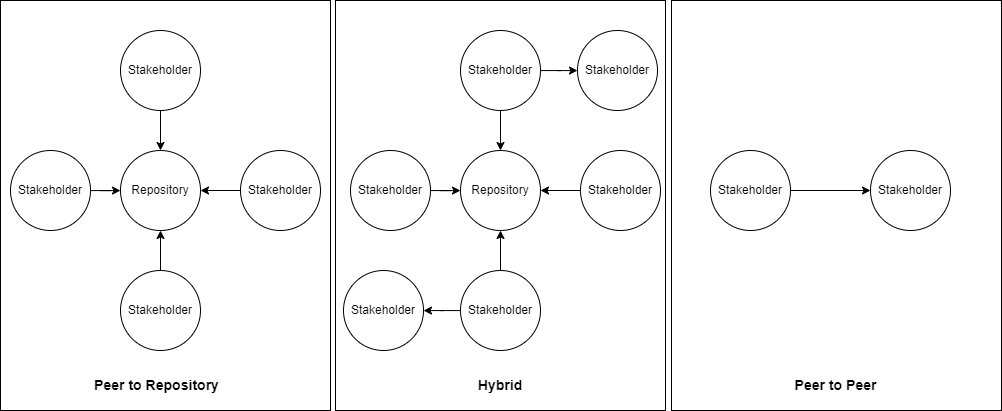
\includegraphics[width=\textwidth]{sharing_models}
    \caption{Information Sharing Models}
    \label{fig:sharing-models}
\end{figure}

In the context of CTI, information sharing can be either peer-to-peer, peer-to-hub (i.e. Repository), or a combination of the two (Figure \ref{fig:sharing-models}). Traditional exchange between two organizations is an example of a peer-to-peer sharing. In the peer-to-hub, a hub or repository is used to collect and distribute data. If the repository is openly accessible to anyone, it is called open source CTI \cite{jesus_sharing_2023}. Jesus et al. \cite{jesus_sharing_2023} investigated the state of the art of the open source CTI and found the barriers that have prevented the formation of any widely used open source CTI platform. 
The barriers mentioned are 1) Legal and regulatory (e.g. GDPR or intellectual property) 2) Interoperability (e.g. different formats) 3) Usefulness and return 4) Market factors (e.g. losing reputation, free-riding) 5) Trust in peers and adversarial usage 6) Confidentiality risks.

After studying these barriers, as well as some technical gaps, they present a confidentiality and privacy analysis of sharing a large sample data set of CTI, to make the claim that it is possible to manage risks of sharing using simple techniques like sanitization. Finally, they propose a set of requirements and a reference architecture for an open source threat intelligence platform. 


\subsection{Current Dataspace Initiatives}
There are several initiatives that are working to create a standard for Dataspaces. The most prominent ones are International Dataspaces (IDS) and Gaia-X. In this section, we will review these two initiatives and compare them.

\paragraph{IDSA}

The International Dataspaces (IDS) is an initiative with the goal of creating a standard for a distributed software architecture for data exchange with sovereignty. It was launched in 2015 as a Fraunhofer research project funded by the German Federal Ministry for Education and Research \cite{otto_evolution_2022}. In 2016, the IDS Association (IDSA) was founded as a non-profit organization to continue the research. It resulted in definition of the IDS Reference Architecture Model (IDS RAM). The IDS RAM is the description of IDS components and their interactions without being technology specific \cite{otto_evolution_2022}. IDS RAM allows anyone to implement the IDS compliant components using any technology. The IDSA also provides a reference implementation of different IDS components called IDS Testbed \footnote{https://internationaldataspaces.org/offers/reference-testbed/}. 

\subparagraph{IDS RAM}
IDS RAM defines the following components \cite{otto_ids_2019}:
Connector, Identity Provider, IDS Broker, Clearing House, IDS Apps, App Store, Vocabulary Provider \cite{pettenpohl_international_2022}.
% \begin{itemize}
%     \item Connector: The connector is the interface between the IDS ecosystem and the data source. It is responsible for the data exchange and the enforcement of the usage control policies as well as authentication.
%     \item Identity Provider: authentication service managing identity information
%     \item IDS Broker: Manages the metadata (description and usage policies)
%     \item Clearing House: Audits the data exchange and manages the payment
%     \item IDS Apps: Process the exchanged data. Deployed within Connector.
%     \item App Store: Provides IDS apps
%     \item Vocabulary Provider: Offers vocabularies to describe and annotate data
% \end{itemize}
Furthermore, it conceptualizes the following roles for the participants:
Data Owner, Data Provider, Data Consumer, Data User, App Provider
\cite{pettenpohl_international_2022}.
% \begin{itemize}
%     \item Data Owner: Controls the data and defines usage policies and payment model.
%     \item Data Provider: Provides the data to the IDS ecosystem with respect to the policies defined by the data owner.
%     \item Data Consumer: Same as data provider but consumes the data.
%     \item Data User: Same as data owner but uses the data.
%     \item App Provider
%     \item ...
% \end{itemize}
% Usage Control:
Also, it defines the standards and procedures to ensure data sovereignty. It uses usage control to enforce the usage policies defined by the data owner. It uses the following components to do so: Usage Control Policy Management Point (UC PMP), Usage Control Policy Decision Point (UC PDP), Usage Control Policy Enforcement Point (UC PEP) \cite{otto_evolution_2022}.
The policies are defined in a machine-readable format which is an extension of the Open Digital Rights Language (ODRL) \cite{eitel_usage_2021}. These policies should be mapped to a specific policy language supported by the tool that enforces them. IDSA RAM mentions the following policy enforcement tools: MYDATA \footnote{https://www.dataspaces.fraunhofer.de/en/software/usage-control/mydata.html}, LUCON \footnote{https://www.dataspaces.fraunhofer.de/en/software/usage-control/lucon.html}, D° \footnote{https://www.dataspaces.fraunhofer.de/en/software/usage-control/d.html}. 
% Certification:
% TODO: Add more details about the certification process


\paragraph{Gaia-X}

Gaia-X is an initiative, launched in 2019, that aims to foster creation of an infrastructure that allows for free and easy exchange of data and services between organizations and evade the vendor lock-in imposed by current proprietary cloud and service providers. To do so, regulations and technical specifications that are based on European values, applicable to any existing cloud and edge technology stack are going to be defined. The goal is to bring transparency, controllability, portability and interoperability across data and services. By facilitating data collection and sharing between organizations, a vibrant data ecosystem across Europe and beyond could evolve. Gaia-X Association deliverables include federation services, common policy rules and an architecture of standards. Federation services can be utilized by the ecosystem participants to achieve a global interoperability, compliance and effortless set up. This includes, “Identity and Trust”, “Federated Catalog” and “Data Exchange services”. \cite{otto_role_2022}
% AISBL: Gaia-X Association
% Nodes, Services (Any cloud service), Service Instances (A service running on a node) and Data Assets (a data set on a node)
% Participants: Organizations and individuals that are part of the Gaia-X ecosystem
% Clearing House: Middle man in the exchange checking for compliance

\paragraph{Comparison of IDS and Gaia-X}

% Mapping of Gaia-X to IDS
    % Federated Catalog ~ IDS Broker + Vocabulary Provider + Information Model
    % Identity and Trust ~ IDS Identity Provider + Dynamic Attribute Provisioning Service (DAPS)
    % Gaia X Sovereign Data Exchange ~ IDS Usage Control and Clearing House
    % Gaia X Node ~ IDS Connector

%  Why choose IDSA? 
    % Maturity
    % Open source Reference Implementation
    % Big picture cloud vs. data exchange

% TODO: 
    % IDSA: usage control
    % Gaia-X: Data at rest

In comparison to IDSA, Gaia-X is less mature and still in the development phase whereas IDSA is used in the industry. It focuses on cloud infrastructures and businesses operating within EU, in contrast to IDSA which is more on the technicalities of the sovereign data exchange. Finally, Gaia-X can use IDSA in the data exchange layer \cite{otto_prof_dr_boris_gaia-x_2021}. 

\paragraph{Other Data Spaces}
Other data management researches based on dataspaces include "Trusted Integrated Knowledge Dataspace For Sensitive Healthcare Data Sharing" (TIKD)  \cite{hernandez_tikd_2021}, which fulfills the following requirements: secure collaborative knowledge graph database of potentially personal data with fine grained access control and privacy-aware data interlinking.
Another example is Real-time Linked Dataspace (RLD) \cite{curry_real-time_2019} which is designed for the Smart Environments, supporting a pay-as-you-go data integration management system for real-time heterogeneous data sources that provides unified query interface based on linked data technologies.
However, these data spaces lack the data sovereignty and usage control features that are necessary for our use case.


% ---------------------------------------------------------------

\section{Use Case and Requirements} % 3 Pages
\label{sec:use-case}

% Scenario
% Requirements
% Constraints

% Two motivations for usage control:
% - Internal: 
% - External: EU-GDPR

% - Confidentiality
% - Security
% - Do we need plausible deniability?
% - Combat against free-riding
% - Trust and reputation

% Some intro about this section
In this section, we will describe the use case and the requirements of the proposed platform. 
% We will also discuss the constraints and limitations of the platform. 
A platform for sharing threat information could be useful for any set of organizations that work together to achieve a common goal who fundamentally use IT systems in their operations. A good platform facilitate creation and operation of sharing communities. Example communities are sector specific ISACs such as ISACs for critical infrastructures, including, energy, water, finance, transportation, and healthcare. In order find concrete requirements, we need to narrow our focus to a specific use case. In this work, we will focus on the energy sector, and more specifically the cyber security of the smart grids.


\subsection{Cyber Security in the Energy Sector}
% TODO: Improve using the new review paper
In order to improve the efficiency of energy distribution grids, efforts are done to make them smart, i.e. smart grids. Smart grids use different information technology (IT) components to collect and process data. However, these components are susceptible to cyber threats. They are an interesting target for attackers, specially advanced state-sponsored attackers, due to the level of damage that is achievable by a successful attack in the energy sector. 

A threat actor for smart grids can be an advanced persistent threat (APT) supported by an enemy government, or a gang of experienced cyber criminals intended to disrupt the energy supply by attacking different actors in the supply chain. By doing so, they can reach their goal of causing a blackout, exfiltrating sensitive information, or gaining financial benefits (e.g. ransomware). 

The important threats that smart grids face are listed by Wallis et al. \cite{wallis_ee-isacpractical_2022}: Data injection attacks on state estimation \cite{deng_false_2019}, distributed denial of service (DDoS) and denial of service (DoS) attacks \cite{wang_coordinated_2019}, targeted attacks, coordinated attacks, hybrid attacks, and advanced persistent threats \cite{leszczyna_cybersecurity_2019}. Moreover, in recent years, ransomware campaigns have emerged as a significant risk to the sector \cite{keshavarzi_i2ce3_2020}.

\subsection{Threat Information Sharing in Energy Sector}

Due to the criticality of the cyber security in the energy sector, organizations in the energy supply chain try to improve their security posture. By using similar technologies, these organizations share the same vulnerabilities. Therefore, they attract the same attackers. These attackers use specific set of tactics, techniques, and procedures (TTP) to attack their victims over and over again. As a result, the victims can prepare themselves for these threats by knowing the TTPs that were used against other victims.

Therefore, energy sector organizations can benefit from sharing threat information with each other. That is where they can use our proposed platform. Therefore, the participants using our platform are different organizations active in the energy supply chain. Here, we assume that participants are the security team of the aforementioned organizations, or a managed security service if the organization does not have its own security team. That is because the security team is the entity responsible for handling the CTI, and we do not consider other types of security information (e.g. logs) in this work.

It is good to note that organizations in the energy sector are subject to the NIS2 directive, therefore they are obliged by the goverment to share cyber security information with other participants in the supply chain and the government.

\subsection{Requirements}
A comprehensive list of requirements requires more research of the existing processes to find the gaps. However, we can foresee that a useful platform should fulfil the requirements structured in the following 3 usage scenarios. 

\paragraph{Scenario 1: Peer to Peer Sharing}
An organization (org 1) after having heard of the platform finds it useful. To join the platform, org 1 passes the necessary certification process. It trusts another organization (org 2) because they also passed the same certification process. They are able to connect to each other because of the interoperability of the different components. They agree to exchange information. To do so, first they negotiate on the scope of exchange and terms and conditions. This can include usage control policies. For example, they agree to only process data in servers located within the EU (to comply with GDPR). Afterwards, they proceed with the actual exchange. 
% First, a committee of decision-making community members should accept the request. Then, after technical certification by the platform admins, B is allowed to join. 


\paragraph{Scenario 2: Share within community}
A utility provider (Acme) has found a new malware in their network. They share the related IOC to their trusted community. They set the usage policy to only allow the data to be read by the participants that have a certain minimum level on a certain trust metric. Furthermore, Acme does not want to share with competing companies. Therefore, it blacklists identified participants that compete in the same market.

\paragraph{Scenario 3: Paid Service and Rating}
% At this point, B should be able to connect to the platform. It should be able to search for available data assets, and fetch metadata. It should explore the existing members and their reputation.
A security organization specialized in selling CTI feeds, wants to use the platform to sell its services. It has a set of CTI feeds that it wants to share with its customers. It wants to charge its customers based on the number of IOCs they receive. Customers are also invited to rate the quality of the feeds they receive. This ratings are used by the customers to choose between different feeds.

% \subsection{Requirements}

% TODO
% Stake-holders (Actors) and their profile
% - Utility Provider
% - Utility Operator (GO)
% - BSI (in Germany) (?)
% - Gov (CERT, CSIRT, BSI)
% - ISAC
% - SMEs
% - SOC (Different Tiers)
% - MSSP (Managed Security Service Provider)

% A use case diagram is shown in figure \ref{fig:use-case}.


% \begin{figure}[ht]
%     \centering
%     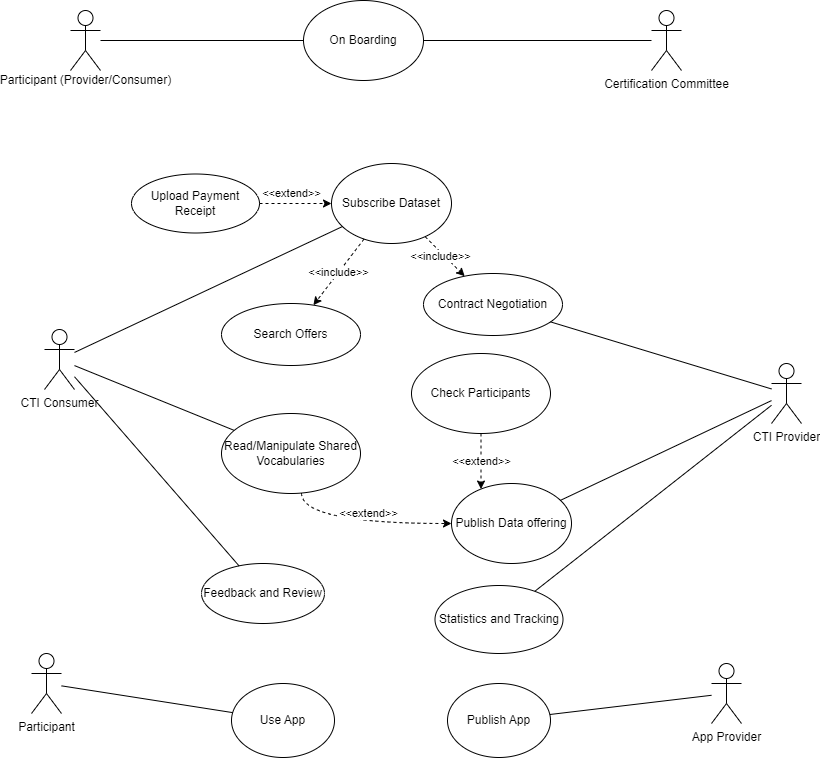
\includegraphics[width=\textwidth]{use_case}
%     \caption{Use Case Diagram}
%     \label{fig:use-case}
% \end{figure}


\section{Conceptual Approach} % 1.5 Pages
\label{sec:conceptual-approach}

% Components and relation to requirements
% Discuss Benefits and limitations
% Compare with existing solutions

\begin{figure}[ht]
    \centering
    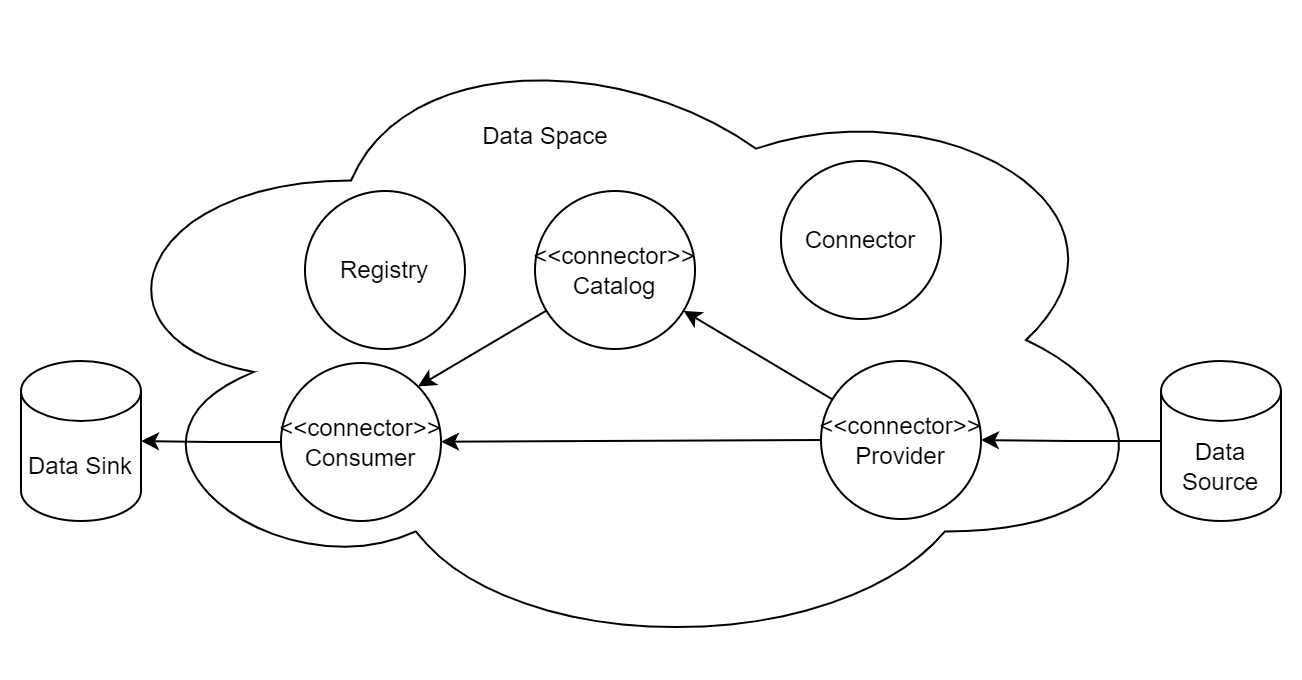
\includegraphics[width=\textwidth]{conceptual_approach.png}
    \caption{System Architecture Diagram}
    \label{fig:system-architecture}
\end{figure}

To support the use case scenarios mentioned, we are going to design and implement a sharing platform based on dataspaces for cyber threat intelligence. A high level diagram is depicted in figure \ref*{fig:system-architecture}. We used a color coding in the diagram: green components are the main contributions of this work. Yellow, are the components that we use or adjust to have a functional prototype. And white components are mentioned in the diagram to show the context, but we are not going to implement them.

\subsection{Dataspace Connector}
We have to set up a functional dataspace to create the backbone of the platform to support sovereign data exchange. It has the ability to handle publishing data offers, secure data exchange, contract negotiation, and enforcing usage policies. Therefore, a dataspace connector component is necessary.

\subsection{Data Modelling}
We need to create data models to be used in the platform. The data models should cover the identified requirements. We expect that we need data models in three different areas:

\paragraph{Usage Policies:} We will specify the formats and data models to express the usage policies based on our requirements, such as prevent access outside EU, or allow only certain fields to be read.

\paragraph*{CTI:} Here we focus on the threat intelligence data that is going to be exchanged. How it will be modeled, using which standard formats, or whether define a new abstract format to support many of existing ones.

\paragraph*{Data Discovery and Negotiation:} Here we should answer the following questions: How one should find published data offers? How to express the search query? After selecting the data, how the negotiation of the contract takes place?

\subsection{Integration with TIP} The sharing platform is only useful when it is integrated to existing tool and platforms for threat intelligence. We should find how data can be extracted from existing threat databases and how the received data could be integrated in the TIP in the data consumer side.

\subsection{Sharing Panel} 
To allow the user of the platform to trigger the necessary functions we need a user interface. The panel is a component that calls the corresponding endpoints in the dataspace connector. It should support the different usage scenarios of the platform, such as searching for offers, negotiation of contracts, specifying usage policies, and uploading the data to the dataspace.

% Important dataspace components that are relevant to our use case are listed below.
% \paragraph*{Connector:} It is the primary component involved in the data exchange acting either as data provider or consumer. Not only it performs the actual data exchange but also the enforcement of the usage control policies as well as authentication. It can be operated on-premises or in a cloud environment. It will run the IDS Apps that do process the data among other things (more on that later). It uses application container management technology to isolate data apps and core functionalities.
% \paragraph*{Broker:} The IDS Metadata Broker is an IDS Connector, which contains an endpoint for the registration, publication, maintenance, and query of Self-Descriptions. Self-Descriptions encapsulate information about Connectors, their managing participant, the offered data assets, and the respective usage conditions. In a sense, the IDS Broker is like a phonebook.
% \paragraph{Clearing House:} It is a trusted third party in the data exchange that logs all the required information about clearing, billing, and usage control. It keeps track of the payment information and also usage information to help verify the compliance with the usage policies.
% \paragraph{Identity Provider:} This is the component serving as Identity and Access Management (IAM). It's responsible for assigning identities to participants, verifying identity claims and granting access based on identities. 
% It comprises three components: 
%         \begin{itemize}
%             \item CAs: One or multiple certificate authorities are responsible for issuing certificates to participants upon request. They are also responsible for revoking certificates. They are the trust anchors by which all other components can be verified.
%             \item Dynamic Attribute Provisioning Service (DAPS): It complements the certificates issued by CAs with more volatile attributes in form of tokens. Connectors can request Dynamic Attribute Tokens (DATs) from DAPS to prove their attributes to other components.
%             \item Participant Information Service (ParIS):  It provides business-related information about participants in the IDS that have been checked by the Support Organization. Similar to the way Broker provides metadata about data assets, ParIS provides metadata about participants.
%         \end{itemize}
%     \item IDS Apps: These are re-usable software components that can be deployed inside the IDS Connector. They are mainly used to transform or analyze data. However, they can also be used to connect to enterprise services, or to allow the connector to be controlled by external systems. Data apps can be chained and bundled.
%     \item App Store: As the name suggests, it is a marketplace for IDS Apps. It contains endpoints to publish, search, and download IDS Apps. It is a Connector on its own, so it should pass the IDS certification criteria and provide a self-description.
%     \item Vocabulary Provider: To facilitate cooperation of different IDS components, a common vocabulary is required. The vocabulary provider enables the participants to define and publish their own vocabularies. Vocabularies typically follow the RDF standard. An example usage is to reference an RDF URI in the Self-Description of a data asset.
% \end{itemize}

% Apart from the components described by the IDS RAM, there are other components that are not part of the IDS RAM but are relevant to our use case. These components are described below.

% \begin{itemize}
%     \item Sanitization App: This is an IDS App that is responsible for sanitizing the data. It is deployed inside the IDS Connector. It is responsible for removing the sensitive information from the data before it is shared with other participants. IDS App is suitable for this task because dealing with sensitive data requires a high level of trust. Apps are certified and verified by the App Store. Furthermore, they are executed within the Connector, so they have access to the data before it is shared with other participants. This is important because it prevents the data from being leaked before it is sanitized. 
% \end{itemize}

\section{Realization / Implementation} % 1 Page
\label{sec:realization}
% Which technology and tools you use?
% Architecture
% - Which parts will you implement yourself, and which part you copy?
%     - IDS Testbed
%     - 

% - How they fit with dataspace components?

\begin{figure}[ht]
    \centering
    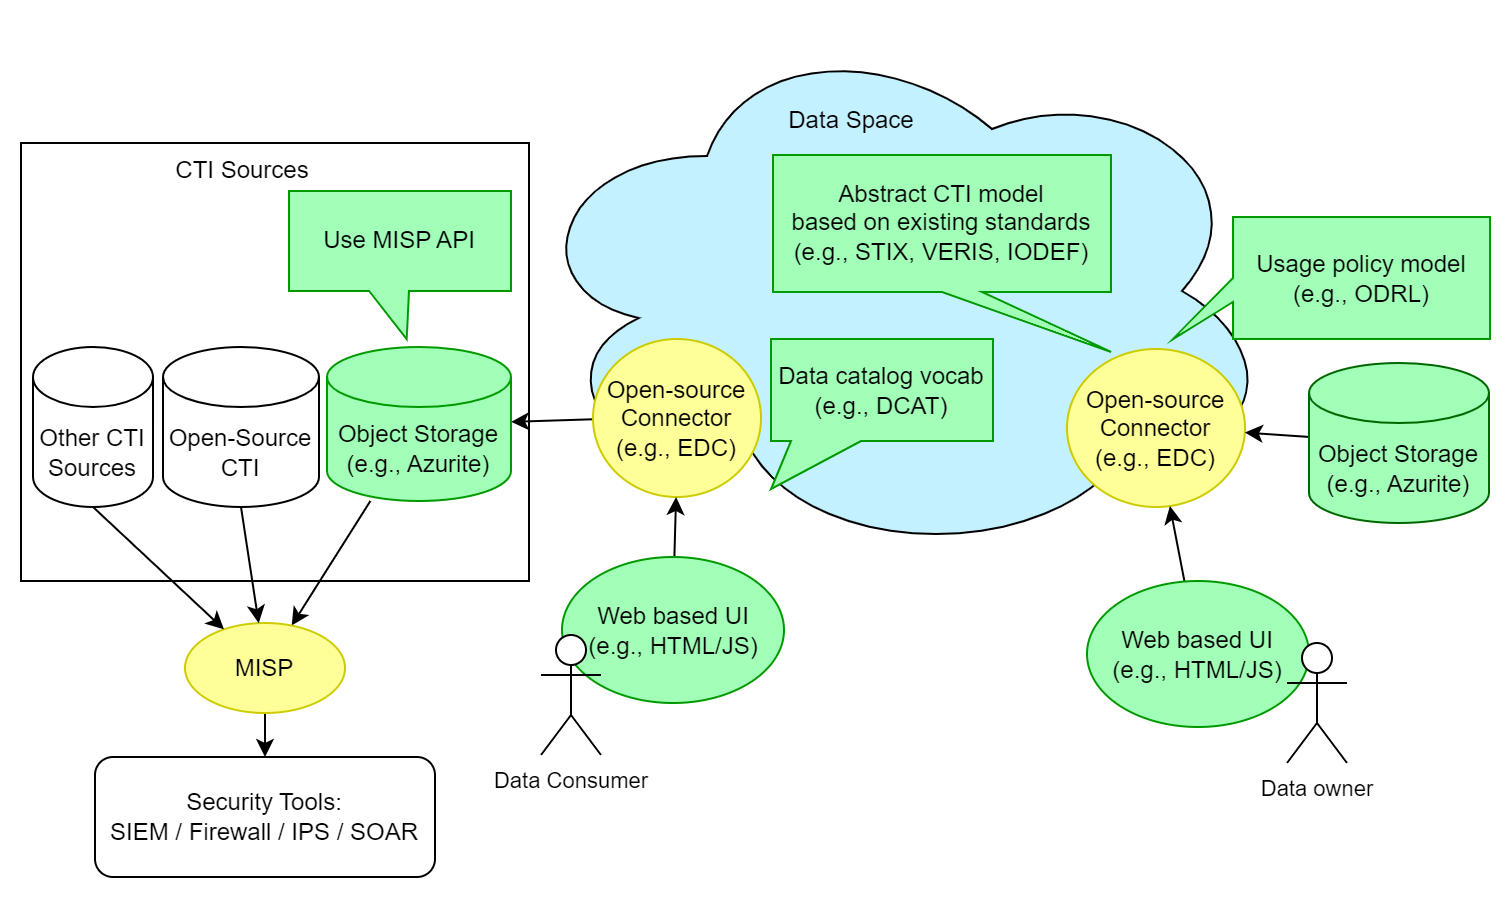
\includegraphics[width=\textwidth]{implementation.png}
    \caption{System Architecture Diagram with Technologies}
    \label{fig:implementation}
\end{figure}


To implement the components mentioned in the last section we are going to use different technologies and tools. An overview is illustrated in figure \ref{fig:implementation}.

\paragraph{Dataspace Connector}
There are different dataspace specifications, but IDS RAM is one that most likely suit our use case.
There are open-source implementations of IDS components such as IDS Connector. An open-source implementation is Eclipse Dataspace Connector (EDC) \footnote{https://github.com/eclipse-edc/Connector}. However, if during the analysis or implementation milestone, we realize that it does not suit our use case, we might switch to simpler solutions such as Solid \footnote{https://solidproject.org}.

\paragraph{Data Modelling}
For expressing the data models we try to stick to the standard formats as much as possible. The result of this task is the vocabularies and ontologies. For usage policies, there are different formats, the most prominent one is ODRL \footnote{https://www.w3.org/TR/odrl-model/}. Also, for the CTI data model we analyze existing standards such as STIX, VERIS, IODEF. Finally, for the data catalogs a common format is DCAT \footnote{https://www.w3.org/TR/vocab-dcat-3/}.

\paragraph{Integration with TIP}
We will an open-source threat intelligence platform, MISP \footnote{https://www.misp-project.org/}, and use its HTTP API to insert the data.

\paragraph{Sharing Panel} The panel is a python script with different arguments for different functionalities. In a real-world scenario it is a graphical user interface which is out of scope of this thesis.

%%%%%%%%%%%%%%%%%%%%%%%%%%%%%%%


% \subsection*{IDS Connector}
% The IDS Association publishes a monthly report of the current state of all the data connectors used for exchange of data, not limited to the IDS compliant connectors.
%  Dam et al. \cite{dam_survey_2023} investigated this report and published a survey in September 2023. They found that only 4 connectors have their source code available on a public repository: 1) IDS Dataspace Connector (DSC) by sovity, Eclipse Dataspace Connector (EDC), the TRUsted Engineering (TRUE) Connector, and the Trusted Connector by Fraunhofer AISEC.

% In addition to that, I found two more: First, IDS Integration Toolbox by Open Logistics Foundation which is a wrapper around the DSC. Second, TNO Security Gateway (TSG) initially developed by TNO which has implementations for many IDS components. It is used in Smart Connected Supplier Network (SCSN) dataspace and has a documentation.
% However, it has no stars on gitlab.

% The overview of different conenctors is shown in table \ref{tab:connectors}.

% \begin{table}[ht]
%     \label{tab:connectors}
%     \centering
%     \begin{tabular}{|c c c c c c|}
%     \hline
%     \textbf{Name} & \textbf{Created} & \textbf{Stars} & \textbf{Commits} & \textbf{Released} & \textbf{Hosted} \\
%     \hline
%     \hline
%     DSC & 07.10.2020 & 27[+101] & 2600 & 10.22 & \href{https://github.com/International-Data-Spaces-Association/DataspaceConnector}{Github} \\
%     \hline
%     EDC & 13.01.2021 & 202 & 1817 & 10.23 & \href{https://github.com/eclipse-edc/Connector}{Github} \\
%     \hline
%     TRUE & 30.10.2020 & 19 & 122 & 08.23 & \href{https://github.com/Engineering-Research-and-Development/true-connector}{Github} \\
%     \hline
%     Trusted & 05.09.2017 & 43 & 2221 & 02.23 & \href{https://github.com/Fraunhofer-AISEC/trusted-connector}{Github} \\ 
%     \hline
%     Toolbox & 31.03.2022 & 3 & 172 & 04.23 & \href{https://git.openlogisticsfoundation.org/silicon-economy/base/ids/ids-integration-toolbox}{Self-Hosted} \\
%     \hline
%     TSG & 12.05.2021 & 0 & 243 & 08.23 & \href{https://gitlab.com/tno-tsg}{Gitlab} \\
%     \hline
%     \end{tabular}
%     \caption{Available IDS Connectors}
% \end{table}

% Most number of stars and most recent release being a deciding factor, I will choose EDC to base my implementation on.

% \subsection*{IDS Testbed}
% The IDS association defines Minimum Viable dataspace (MVDS) as the minimum set of components that provide the ability to do secure and sovereign data exchange. They specify the required components as follows: Two Connectors (a data provider and a consumer), an Identity Provider (Dynamic Attribute Provisioning Service, Certificate Authority). IDSA has published an open-source project, \href{https://github.com/International-Data-Spaces-Association/IDS-testbed}{IDS Testbed}, that contains instructions to install and orchestrate these set of minimum components. It references open-source implementations of these components, see table \ref{tab:components} to find source code of these components.

% \begin{table}[ht]
%     \label{tab:components}
%     \centering
%     \begin{tabular}{|c|c|c|c|}
%     \hline
%     \textbf{Component} & \textbf{Source Code} & \textbf{Version} & \textbf{Language} \\
%     \hline
%     IDS Testbed & \href{https://github.com/International-Data-Spaces-Association/IDS-testbed}{Testbed Git} & 1.0 & Docker-Compose \\
%     \hline
%     Connector & \href{https://github.com/International-Data-Spaces-Association/DataspaceConnector/tree/v8.0.2}{Connector Git} & 8.0.2 & Java \\
%     \hline
%     Metadata Broker & \href{https://github.com/International-Data-Spaces-Association/metadata-broker-open-core}{Broker Git} & 5.0.3 & Java \\
%     \hline
%     DAPS & \href{https://github.com/International-Data-Spaces-Association/omejdn-daps}{DAPS Git} & 1.6.0 & Ruby \\
%     \hline
%     Certificate Authority & \href{https://github.com/International-Data-Spaces-Association/IDS-testbed/tree/master/CertificateAuthority}{Testbed Git} & --- & Python \\
%     \hline
%     App Store & \href{https://github.com/International-Data-Spaces-Association/IDS-AppStore}{App Store Git} & 3.0.0 & Java \\
%     \hline
%     \end{tabular}
%     \caption{Necessary Components}
% \end{table}

% In addition to the aforementioned components, some new ones need to be implemented from scratch: App Store, ParIS, Clearing House, Vocabulary Hub. Of course, the required IDS Apps should be implemented, which includes, the Sanitization App. 
% For the App Store there is a published project (\href{https://github.com/International-Data-Spaces-Association/IDS-AppStore}{App Store Git}) which is not included in the testbed and might not be fully functional.

% \subsection*{Usage Policies}
% To describe usage policies IDS defines its own Usage Control Language which is an extension of Open Digital Rights Language (ODRL). It is a machine readable format which is technology agnostic. There are multiple mechanism to enforce these policies automatically. The position paper on IDS Usage Control \cite{eitel_usage_2021} lists the following mechanisms: MYDATA Control Technologies, Logic based Usage Control (LUCON), and Degree (D°). According to the paper, MYDATA Control Technologies is the most mature and comprehensive. It is also the only one that is implemented in the IDS Testbed. Therefore, I will use MYDATA Control Technologies to enforce the usage policies. The usage control is enforced in the IDS Connector possibly using a separate application container. It comprises three different components: PMP, manages policies and creating them based on some templates, PDP, evaluates the policies and decides whether to allow or deny the request, and PEP, enforces the decision made by PDP. The overview of the components is shown in figure \ref{fig:connector}.

% \begin{figure}[ht]
%     \centering
%     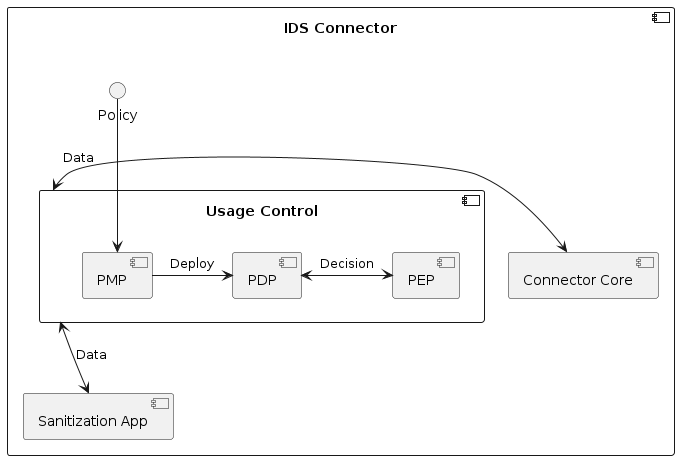
\includegraphics[width=\textwidth]{connector}
%     \caption{Connector Overview}
%     \label{fig:connector}
% \end{figure}


% \subsection*{Sanitization App}
% Removing all sensitive data from CTI in general can be a difficult task. There are different CTI formats and each format has its own structure. Furthermore, deciding whether a value contains confidential information or not is not straight-forward. Even a sophisticated machine learning approach requires a lot of data with different types of confidential information to be trained on. Therefore, I will focus on creating a base sanitization app that is easily extensible to detect more sensitive data. To start, it should support sanitizing JSON based CTI formats, and a configurable set of regex rules to detect sensitive data. Refining this app to support more formats and more sophisticated detection mechanisms is out of scope of this thesis.

\section{Evaluation} % 0.5 Page
\label{sec:evaluation}
% Methodology and Metrics
% Test scenario

% - How to gather (CTI) data?
% - Metrics for evaluating the privacy? (e.g. entropy)
% - The steps of the scenario and the expected results
% - How to measure the performance?

The evaluation is consisted of two approaches, analytical and experimental. In the analytical approach, we will go through the identified requirements and validate the designed architecture against them, to measure the extent to which the requirements are fulfilled. Moreover, will dive deeper in the security and privacy requirements and perform a comparative analysis against our baseline, MISP. We will also take a look at the threats in the energy sector and see how our platform could mitigate them.

The experimental approach is based on simulations using the created prototype. By executing different use case scenarios on the prototype we can validate qualitively the effectiveness of the platform in action and see how the requirements are satisfied. We can also measure quantitively some performance metrics such as throughput, delay and resource consumption. Similar to the analytical approach, we dive deep in the security and privacy requirements and simulate some attack vectors and see how the platform can help defend against them.

% My contribution being design of a sharing platform for CTI data, the evaluation should measure the effectiveness of the sharing platform. The problem is that according to my research, there is no benchmark available and no defined metrics to this aim. Having no baseline to compare against, it seems hard to reach an objective evaluation. Furthermore, many performance metrics depend on the implementation, infrastructure, and the details of the scenario. Since, my main contribution is the design of the platform, not the implementation, some metrics can be misleading. 

% However, several options can be thought of. First, by focusing on the main effect of using dataspaces for data sharing, which is the addition of usage control and changing the data flow, one can define a few specific metrics. Having defined some usage case scenarios and a sample implementation, we can measure for example the following metrics: 
% \begin{itemize}
%     \item Number of unnecessary participants that should have access to the data.
%     \item The difficulty of changing the usage policies.
%     \item How difficult it is to revoke access to the data.
%     \item Variety of types of usage policies that are enforceable.
%     \item How many scenarios are significantly improved using our approach.
% \end{itemize}

% The above-mentioned items might be subjective and change by modifying the chosen scenarios, but investigating it can provide some insights into the effectiveness of the dataspaces.

% Another approach which can sound more objective is to design a survey. It should use some standard templates to be comparable. The survey should be conducted on a group of experts in the field of threat information sharing after presenting them our approach. The survey should be designed to measure the effectiveness of our design in terms of privacy and security. Ideally, 10 to 20 experts should be interviewed. There is a risk of not having enough experts available. In that case, we fall back to the first approach.


\section{Project Plan} % 0.75 Page
\label{sec:timeline}

The work is planned to take 6 month (26 weeks), and consists of 5 Milestones:

\paragraph*{Milestone 1 (1 Dec - 21 Dec: 3 weeks): Foundation} 
    \begin{itemize}
        \item Related work: Review the related works
        \item Define use case scenarios: Find concrete scenarios and requirements
    \end{itemize}
\paragraph*{Milestone 2 (21 Dec - 12 Jan: 3 weeks): Analysis and Modelling}
    \begin{itemize}
        \item Information Modelling: Define required data models
        \item System Design: Specify the components and the data flows
    \end{itemize}
\paragraph*{Milestone 3 (12 Jan - 9 Mar: 7 weeks): Prototype Implementation}
    \begin{itemize}
        \item Setup Dataspace: Implement the components for the dataspace
        \item Integration with TIP
        \item Sharing Panel
    \end{itemize}
\paragraph*{Milestone 4 (9 Mar - 7 Apr: 4 weeks): Evaluation}
\paragraph*{Milestone 5 (7 Apr - 29 May: 7 weeks): Writing and buffer}

\bibliography{References} 
\bibliographystyle{ieeetr}

\end{document}
